\documentclass[12pt]{article}
\usepackage[margin=1.25in]{geometry}
\usepackage{grt}
\usepackage{changepage}
\usepackage{graphicx}
\usepackage{tikz}
\usepackage{hyperref}
\usepackage{xcolor}
\usepackage{listings}
% \usepackage{algorithmic}

\definecolor{codegreen}{rgb}{0,0.6,0}
\definecolor{codegray}{rgb}{0.5,0.5,0.5}
\definecolor{codepurple}{rgb}{0.58,0,0.82}
\definecolor{backcolour}{rgb}{0.95,0.95,0.92}
 
\lstdefinestyle{mystyle}{
    backgroundcolor=\color{backcolour},   
    commentstyle=\color{codegreen},
    keywordstyle=\color{magenta},
    numberstyle=\tiny\color{codegray},
    stringstyle=\color{codepurple},
    basicstyle=\ttfamily\footnotesize,
    breakatwhitespace=true,         
    breaklines=true,                 
    captionpos=b,                    
    keepspaces=true,                 
    numbers=left,                    
    numbersep=5pt,                  
    showspaces=false,                
    showstringspaces=false,
    showtabs=false,                  
    tabsize=4
}
 
\lstset{style=mystyle}

\newcommand{\prob}{\operatorname{Prob}}

\begin{document}
\begin{center}
    \Large{Reconstructing Phylogenies with Variable Evolution Rates Among Sites} \\
    \vspace{0.5cm}
    \normalsize{Garrett Tetrault, grt43}
\end{center}

\sectionline

\subsection*{Introduction}
    In the phylogenetic models we have developed in class, there have been drastic simplifications to allow for easy understanding and computation.
    One principle simplification has been the assumption that each site in the genetic sequences evolves at the same rate.
    For example, there may be several conserved regions in the sequences with only a subset of regions displaying significant change.
    This is what is captured by modeling different rates of evolution.
    In this paper, I will focus on the following paper by Felsenstein and Churchill
    that presents a model to compute the likelihood of a phylogeny,
    allowing for unequal evolutionary rates at different sites in the molecular sequences.
    \begin{adjustwidth}{1in}{1in}
        J Felsenstein, G A Churchill, 
        A Hidden Markov Model approach to variation among sites in rate of evolution., 
        Molecular Biology and Evolution, Volume 13, Issue 1, Jan 1996, Pages 93–104, \\
        \url{https://doi.org/10.1093/oxfordjournals.molbev.a025575}
    \end{adjustwidth}
    We will begin by describing the model and likelihood calculations, then transition to examining how different sets of evolutionary rates effect a phylogenies likelihood and its maximum likelihood assignment of evolutionary rates.

\subsection*{Evolution Rate Model}
    At the core of the model developed by Felsenstein and Churchill is a Hidden Markov Model that describes the changes in evolutionary rates at each possible site in the different DNA sequences in a given phylogeny.
    Each node in the model corresponds to a different rate of evolution with transitions between all possible states.
    For example, consider the set of evolutionary rates $\set{10.0, 2.0, 0.3}$. 
    A Hidden Markov Model for their model must be of the form,
    \begin{center}
        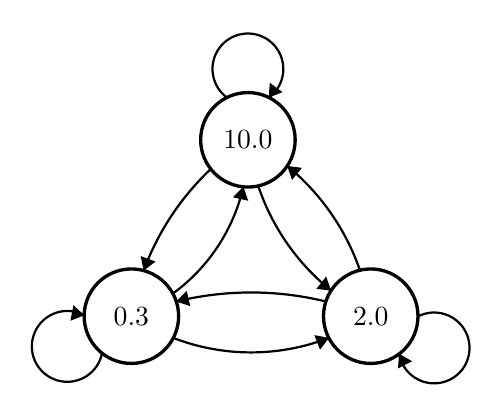
\begin{tikzpicture}[scale=0.2]
        \tikzstyle{every node}+=[inner sep=0pt]
        \draw [black, very thick] (39.1,-21.8) circle (3);
        \draw (39.1,-21.8) node {$10.0$};
        \draw [black, very thick] (46.9,-33) circle (3);
        \draw (46.9,-33) node {$2.0$};
        \draw [black, very thick] (31.7,-33) circle (3);
        \draw (31.7,-33) node {$0.3$};
        \draw [black, thick] (38.812,-24.778) arc (-12.9237:-53.98292:11.603);
        \fill [black, thick] (38.81,-24.78) -- (38.15,-25.45) -- (39.12,-25.67);
        \draw [black, thick] (44.385,-31.375) arc (-128.82003:-161.47106:14.42);
        \fill [black, thick] (44.38,-31.38) -- (44.07,-30.48) -- (43.45,-31.26);
        \draw [black, thick] (34.549,-32.068) arc (103.79463:76.20537:19.926);
        \fill [black, thick] (34.55,-32.07) -- (35.44,-32.36) -- (35.21,-31.39);
        \draw [black, thick] (37.777,-19.12) arc (234:-54:2.25);
        \fill [black, thick] (40.42,-19.12) -- (41.3,-18.77) -- (40.49,-18.18);
        \draw [black, thick] (29.838,-35.338) arc (-10.79888:-298.79888:2.25);
        \fill [black, thick] (28.71,-32.94) -- (28.02,-32.3) -- (27.83,-33.29);
        \draw [black, thick] (49.888,-33.018) arc (117.38552:-170.61448:2.25);
        \fill [black, thick] (48.7,-35.38) -- (48.63,-36.32) -- (49.52,-35.86);
        \draw [black, thick] (41.596,-23.456) arc (50.64661:19.0623:14.842);
        \fill [black, thick] (41.6,-23.46) -- (41.9,-24.35) -- (42.53,-23.58);
        \draw [black, thick] (32.48,-30.107) arc (159.80586:133.28752:16.866);
        \fill [black, thick] (32.48,-30.11) -- (33.23,-29.53) -- (32.29,-29.18);
        \draw [black, thick] (44.242,-34.378) arc (-68.86222:-111.13778:13.705);
        \fill [black, thick] (44.24,-34.38) -- (43.32,-34.2) -- (43.68,-35.13);
        \end{tikzpicture}
    \end{center}

    Below, we have a visual depiction of how the aforementioned Hidden Markov model can be used to describe site-wise differences in evolutionary rate,
    \begin{center}
        \includegraphics[scale=0.25]{../figs/hmm_model.png} \\
        \small{Image taken from original paper.}
    \end{center}
    This model has some important implications.
    Chiefly, it supposes we have some preconceived notion of how a finite set of evolutionary rates relate to one another in a Hidden Markov Model.
    That is, as input, the model requires the different rates $\set{r_i}$ to be known and the transition probabilities $P_{ij}$ from rate $r_i$ to rate $r_j$ to be known as well.
    Secondly, as a result of the use of a Hidden Markov Model, each site evolves independently from all other sites apart from that directly preceding it.
    In practice, and in our implementation, it is much easier to use the equilibrium probabilities of each rate instead of specifying each transition probability.
    We will denote $f_i$ to be the equilibrium probability of rate $r_i$.
    As a further piece of notation, we will use $c_k$ to denote the rate category (node in Hidden Markov Model) of the underlying rate $r_i$ at site $k$.

\subsection*{Likelihood Calculations}
    The crux in a model like this is formulating a way to compute its likelihood given some phylogeny.
    We will assume we are given sequence data $D$ and some tree topology $T$.
    Below, we state the formulation that was derived by Felsenstein and Churchill.
    Let $L$ be the likelihood of the model, 
    and $L_{c_k}^{(k)}$ be the likelihood of $T$ for the data consisting of sites $k$ through $n$
    given that site $k$ has rate category $c_k$.
    Then we have,
    \begin{gather*}
        L = \sum_{c_1}f_{c_1}L_{c_1}^{(1)} \\
        L_{c_k}^{(k)} = 
            \prob(D_k \mid T, r_{c_k})
            \sum_{c_{k+1}}P_{c_k, c_{k+1}}f_{c_{k+1}}L_{c_{k+1}}^{(k+1)} \\
        L_{c_n}^{(n)} = 
            \prob(D_n \mid T, r_{c_n})
    \end{gather*}
    What is interesting to note is that this model is computing the likelihood of all possible combinations of rates at each site, not just some optimal sequence of rates.

    Methods were also developed to recover the most likely sequence of rates.
    Let $R_{c_k}^{(k)}$ be the likelihood contribution for sites $k$ through $n$ 
    with site $k$ having rate category $c_k$, 
    and sites $k+1$ through $n$ having some combination of categories that maximizes the contribution of sites $k$ through $n$.
    We then have that,
    \begin{gather*}
        R_{c_k}^{(k)} = 
            \prob(D_k \mid T, r_{c_k})
            \max_{c_{k+1}}\set{P_{c_k, c_{k+1}}f_{c_{k+1}}L_{c_{k+1}}^{(k+1)}} \\
        R_{c_n}^{(n)} = 
            \prob(D_n \mid T, r_{c_n})
    \end{gather*}
    Let $c_1$ be the rate that maximizes the value of $R_{c_1}^{(k)}$.
    If we store the sequence $\set{c_k}$ that is chosen in the maximizing steps, 
    we can recover the maximal likelihood sequences backtracking over our choices
    in a process that is very similar to the Viterbi algorithm.

    In both of these computations we must compute $\prob(D_k \mid T, r_{c_k})$.
    Below, we have an expression for this value assuming we are using the Jukes-Cantor model of evolution (which we will do for our implementation).
    First, let $\ell_{ic}^{(m)}(b)$ be the likelihood of $T$ for all data for site $m$ at or above node i on the tree, given that site $m$ in node $i$ is basis $b$, and given that site $m$ has rate category $c$.
    As the calculation of this value is exactly that in Felsenstein's algorithm, we will not be stating directly its formulation.
    Let $M_{xy}(v, r)$ denote the site-wise evolution model (in this case Juke-Cantor) that denotes the probability of transitioning from basis $x$ to basis $y$ with a branch length of $v$ and evolutionary rate $r$.
    With this, we then have that,
    \[
        \prob(D_i \mid T, r_{c_i}) 
        = \frac{1}{4}\sum_x \sum_y \ell_{jc_i}^{(i)}(x) M_{xy}(v, r_{c_i}) \ell_{kc_i}^{(i)}(y).
    \]
    We are now well-equipped to implement to the model.

\subsection*{Implementation Details}
    As we have mentioned, we will be using the Juke-Cantor model of evolution in our implementation.
    This is a departure from the more complex Hasegawa, Kishino and Yano model used in the paper's implementation.
    Additionally, we have set our transition probabilities to be,
    \[
        P_{ij} = \lambda \delta_{ij} + (1 - \lambda)f_{j}.
    \]
    Here, $\lambda$ is an `autocorrelation' parameter such that the average expected patch length is $\sfrac{1}{(1 - \lambda)}$. 
    This is set by the user.

    For data, we turn to the USCS genome browser.
    Specifically, we are examining the $\beta$-hemoglobin DNA sequences.
    We use the following species,
    \begin{adjustwidth}{1in}{1in}
        \{human, gorilla, chimp, gibbon, green monkey, golden snub-nosed monkey,and orangutan\}
    \end{adjustwidth}
    To obtain a phylogeny from this, we use the PHYLIP software package implemented by Felsenstein and use this to input a tree topology and branch lengths into our model.

\subsection*{Results}
    Below, we have the phylogeny returned to us by the PHYLIP package,
    \begin{center}
        \includegraphics[scale=0.5]{../figs/phylo.png}
    \end{center}
    We will now begin examining different rates of evolutions and different equilibrium probabilities.
    Note that the evolution rates specified were attained from experimentation.
    There appeared to be a threshold for the evolutionary rates for this data set around $0.75$ at which the chance of selecting the evolutionary rate was extremely low.
    This stands to reason as we are working only with primate species and would expect them to be evolutionarily similar.

    For the first analysis, we will set the auto-correlation parameter to be $\lambda=0.9$.
    As a base line, we first compute the likelihood of the model with a flat evolutionary rate of $0.3$.
    With this, we find a log likelihood of \texttt{-64420.0656448217}.

    We first split the evolutionary rates into a high rate of $0.4$ and a low rate of $0.2$,
    with equal equilibrium probabilities.
    That is, $f_i = 0.5$ for $i \in {\ntxt{Low},\ntxt{High}}$.
    With these conditions we find that the log-likelihood is \texttt{-64569.30264119623}.
    To visualize this, we plot the rate categories as shading regions and differences in bases among sequences below,
    \begin{center}
        \includegraphics[scale=0.5]{../figs/high_low.png}
    \end{center}

    We now allow for a third evolutionary rate model of $0.3$.
    We first test the results when the equilibrium probabilities are all equal.
    That is, $f_i = 0.333$ for $i \in {\ntxt{Low},\ntxt{Medium}, \ntxt{High}}$.
    With these conditions we find that the log-likelihood is \texttt{-64480.19948628911}.
    To visualize this, we plot the rate categories as shading regions and differences in bases among sequences below,
    \begin{center}
        \includegraphics[scale=0.5]{../figs/high_med_low.png}
    \end{center}

    We now examine what happens when we wildly change the equilibrium probabilities.
    We will let $f_{\ntxt{Low}} = 0.8$ and $f_{\ntxt{Medium}} = f_{\ntxt{High}} = 0.1$.
    With these conditions we find that the log-likelihood is \texttt{-64571.29739397782}.
    To visualize this, we plot the rate categories as shading regions and differences in bases among sequences below,
    \begin{center}
        \includegraphics[scale=0.5]{../figs/high_med_low_weighted_low.png}
    \end{center}

    From this we can see that, even if we weight the preference greatly towards a specified evolutionary rate, the dominant rate, in this case the Medium rate, will still be the most apparent.
    Interestingly, these results indicate that the model was most likely (in our tests) with a static evolution rate of $0.3$.
    This could be potentially due to, again, the fact that these species are fairly closely related and that we are working on the same protein.

    Returning to the model in which we have a high, medium, and low rates of $0.4$, $0.3$, and $0.2$ respectively with equal equilibrium probabilities.
    Now, however, we will examine different autocorrelation parameters.

    We begin with $\lambda = 0.2$.
    With these conditions we find that the log-likelihood is \texttt{-64482.77727355491}.
    To visualize this, we plot the rate categories as shading regions and differences in bases among sequences below,
    \begin{center}
        \includegraphics[scale=0.5]{../figs/high_med_low_low_lambda.png}
    \end{center}

    We now consider $\lambda 0.5$.
    With these conditions we find that the log-likelihood is \texttt{-64481.185185916955}.
    To visualize this, we plot the rate categories as shading regions and differences in bases among sequences below,
    \begin{center}
        \includegraphics[scale=0.5]{../figs/high_med_low_medium_lambda.png}
    \end{center}

    As would be expected, we can see that varying $\lambda$ determines the probability we can transition from one state to another.
    In the case of a very low $\lambda$, we are seeing the evolution rates over fit the data, switching at nearly every position.

\subsection*{Extensions}
    A significant extension to this project would be to use the likelihood calculations to determine the maximum likelihood phylogeny.

\begin{lstlisting}
(1) Begin with one DNA sequence.

(2) For each subsequent sequence:

    (3) For each possible edge to join on tree:

        (4) Compute the maximum likelihood branch length 
        by Newton's Method.

        (5) Compute the likelihood of the tree with the 
        new sequence and branch.

    (6) Keep the maximum likelihood tree topology and 
    branch lengths.

(7) Return the final tree topology. \end{lstlisting}
    To compute the maximum likelihood branch length, first recall the basic structure of Newton's Method.
    Let $(j,k)$ be the new edge we are adding.
    Consider likelihood as a function of the branch length $L(v)$.
    To maximize, we find $v$ such that $\frac{dL}{dv} = 0$.
    This is done by a recursive formula that approaches a value where this is true.
    That recursive rule is,
    \begin{gather*}
        v_{i+1} = v_i - \left( \frac{dL}{dv}(v_i) \left/ \frac{d^2L}{dv^2}(v_i) \right. \right)
    \end{gather*}
    These derivatives can be computed from straight forward calculations of the previous formulas.
    The paper outlines how they can be computed for their model, however as we have mentioned, they used the Hasegawa, Kishino and Yano model as opposed to the Jukes-Cantor model.
    In the Jukes-Cantor model, the derivatives are given by,
    \[
        \frac{dL}{dv} = \sum_{c_1}f_{c_1}\frac{dL_{c_1}^{(1)}}{dv}
    \]
    \begin{align*}
        \frac{dL_{c_k}^{k}}{dv} 
        =& \left( \frac{d\prob(D_k \mid T, r_{c_k})}{dv}
            \sum_{c_{k+1}}P_{c_k, c_{k+1}}f_{c_{k+1}}L_{c_{k+1}}^{(k+1)} \right. \\
        &\quad \left. + \prob(D_k \mid T, r_{c_k})
            \sum_{c_{k+1}}P_{c_k, c_{k+1}}f_{c_{k+1}} \frac{dL_{c_{k+1}}^{(k+1)}}{dv} \right)
    \end{align*}
    \[
        \frac{dL_{c_n}^{(n)}}{dv} = \frac{d\prob(D_n \mid T, r_{c_n})}{dv}
    \]
    and,
    \[
        \frac{d^2L}{dv^2} = \sum_{c_1}f_{c_1}\frac{d^2L_{c_1}^{(1)}}{dv^2}
    \]
    \begin{align*}
        \frac{d^2L_{c_k}^{k}}{dv^2} 
        =& \left(\frac{d^2\prob(D_k \mid T, r_{c_k})}{dv^2}
            \sum_{c_{k+1}}P_{c_k, c_{k+1}}f_{c_{k+1}}L_{c_{k+1}}^{(k+1)}\right. \\
        &\quad+2\frac{d\prob(D_k \mid T, r_{c_k})}{dv}
            \sum_{c_{k+1}}P_{c_k, c_{k+1}}f_{c_{k+1}}\frac{dL_{c_{k+1}}^{(k+1)}}{dv} \\
        &\quad\left.+\prob(D_k \mid T, r_{c_k})
            \sum_{c_{k+1}}P_{c_k, c_{k+1}}f_{c_{k+1}} \frac{d^2L_{c_{k+1}}^{(k+1)}}{dv^2}\right)
    \end{align*}
    \[
        \frac{d^2L_{c_n}^{(n)}}{dv^2} = \frac{d^2\prob(D_n \mid T, r_{c_n})}{dv^2}
    \]
    To compute the site-wise likelihood derivatives,
    we recall that with the Jukes-Cantor model,
    \[
        \prob(D_i \mid T, r_{c_i})
        = e^{-\frac{4}{3}vr_{c_i}}K_1 + K_2
    \]
    where
    \begin{gather*}
        K_1 = \frac{1}{4}\sum_x \sum_y 
            \ell_{jc_i}^{(i)}(x) \left(\delta_{xy} - \frac{1}{4}\right) \ell_{kc_i}^{(i)}(y) \\
        K_2 = \frac{1}{16}\sum_x \sum_y 
            \ell_{jc_i}^{(i)}(x) \ell_{kc_i}^{(i)}(y)
    \end{gather*}
    From this, we can derive the derivatives as follows,
    \begin{gather*}
        \frac{d\prob(D_i \mid T, r_{c_i})}{dv} = -\frac{4}{3}r_{c_i}e^{-\frac{4}{3}vr_{c_i}}K_1 \\
        \frac{d^2\prob(D_i \mid T, r_{c_i})}{dv^2} = \left(\frac{4}{3}r_{c_i}\right)^2e^{-\frac{4}{3}vr_{c_i}}K_1
    \end{gather*}
    One would now have all the analytical pieces for computing steps (4) and (5) in the aforementioned algorithm.
    Due to the time constraints and the complexity of these calculation (particularly in log-space), they have not been implemented in this project.
    However, this extended project would provide a more robust self-contained analysis of phylogenetic trees.

\subsection*{References}
    \begin{enumerate}
    \item 
        \begin{adjustwidth}{0.1in}{1in}
            J Felsenstein, G A Churchill, 
            A Hidden Markov Model approach to variation among sites in rate of evolution., 
            Molecular Biology and Evolution, Volume 13, Issue 1, Jan 1996, Pages 93–104, \\
            \url{https://doi.org/10.1093/oxfordjournals.molbev.a025575}
        \end{adjustwidth}

    \item 
        \begin{adjustwidth}{0.1in}{1in}
            Durbin, Richard et al. “Biological Sequence Analysis: Probabilistic Models of Proteins and Nucleic Acids.” (1998).
        \end{adjustwidth}
    \end{enumerate}

\newpage
\subsection*{Code}
    \texttt{phylogeny.py}
    \lstinputlisting[language=Python]{../src/phylogeny.py}

    \newpage
    \texttt{main.py}
    \lstinputlisting[language=Python]{../src/main.py}

\end{document}